\documentclass[]{article}
\usepackage{listings}
\usepackage{graphicx}
\usepackage{float}
\setlength\parindent{0pt}
\setlength{\parskip}{1em}
%opening
\title{Visualizing High-dimensional Ball-Embeddings
	while Keeping Topological Relations}
\author{Jan Scheffczyk \\ Oliver Leuschner \\ Joanna Polewczyk}
%

\begin{document}

\maketitle

%150-250 words
%
%
%
\newpage
\section{Introduction}



\section{N-Balls embeddings}
\label{sec::ball}
Hierarchies or in other words trees can be expressed by ball embeddings. The largest N dimensional sphere corresponds to the root node of the tree. The direct children of the root node are represented by smaller spheres that are contained within the sphere of the root node. Hierarchies are an important part of natural language and signify a type of relationship with another word. For example sparrow, duck or Eagle are all of the type bird. In linguistics this is called a hypernym and hyponym relationship where the type of, in our example the bird, would be the hypernym and the concrete realizations of that type, in our example sparrow or a duck, would be some of the hyponyms of bird. It is evident that having this kind of hierarchical information can be useful when creating a rule-based natural language processing tool. Unlike stochastic or learning based methods hierarchical structures do not have error term to be minimized. Hierarchical structures are deterministic meaning we can always determine if a note is a child (hyponym) of a word that we are interested in or not. For example if we were to write a tool that needs to identifies cities within a certain region then the results certainly have to be direct or indirect hypnonyms of the word city.
\par
While rule-based natural language processing methods have been studied and applied for many decades recent machine learning algorithms, specifically deep neural networks, have produced stunning results that seemed almost impossible with the traditional rule-based approaches. However to actually use words or sentences in a neural network we first have to convert the input into to a vector that we can train our model on. This was first popularized in the word2vec paper. The goal is to create a dense vector representation for each word. The authors start off by creating a sparse representation also known as one hot encoding. For this they determine all words used in their text corpus and create a vocabulary from that. Then every word can be represented by a vector of the length of the vocabulary that only contains a single entry of 1 and all of the other entries are 0. This allows us, though in a very inefficient way, to feed any word or even a sentence, a concatenation of these vectors, into a neural network. Further they assume that similar words have a similar context. For example in "Can you *blank* me the train station." we can fill this gap with \textit{lead, guide,show} and all of them express a similar meaning. We can then train a neural network to represent every word with a limited dimension of our choosing. Common vector dimensions are 50, 100,300,500. This works remarkably well and allows us to explore relationships beyond simple hierarchies. In the original paper they could use the word vectors for simple arithmetics, one example of this would be Paris-France+ Italy=Rome. This approach has been extended multiple times, one such instance are the GloVe word embeddings. As with all learning based methods there is no guarantee that certain relationships that we observe in our language are actually projected into the word vector space. 

N-Ball embeddings combine both approaches and fuse the reliability of a hierarchical based system with the power and flexibility that  word vectors provide. This is achieved by extending the word vectors and conceptually adding a sphere to each of them. In the next step we need to ensure that the word embeddings actually adhered to the hierarchical structure that we want to embed into them while preserving the vector that has been assigned by the word embedding of our choice. This is done by adding more dimensions to these word vectors and then only performing homothetic transformations on them.

\section{The Architecture}
\label{sec::arch}
Here we will describe the basic information flow between the user interface given on the website, the Web server as well as the way request are handled. In order to display any kind website we first need to set up a Web server that serves HTML files along with their corresponding CSS and JavaScript files. As discussed previously we chose to use flask for this task as it allows us to stay in the Python ecosystem. We created a basic HTML website that provides a input field as well as some basic information about the project so that the user can understand the idea of the project and then proceed to either execute the given example or come up with his own. 
The user provides a tree structure which he would like to embed into a  embedding. Using statements with a fixed structure
\begin{center}
	
\begin{tabular}{c}
\begin{lstlisting}
Enity_1 is Enity_2
Enity_1 is NOT Enity_2
\end{lstlisting}
\end{tabular}
	
for example
	
\begin{tabular}{c}
\begin{lstlisting}
chicken  is animal
human    is animal
socrates is human
tank     is NOT animal
kant     is human
		
\end{lstlisting}
\end{tabular}
\end{center}
provide a simple way to describe a single hypernym or hypnoym relationship in a form that is both human readable and can be easily parsed internally. Instead of using the input field users can also upload a text file where each line contains a single hypernym statement. While this does provide a good way to intuitively define small tree structures we have to make a few assumptions in order to do the actual visualization. Both the underlying word vectors as well as the algorithm to create the N ball embedding is now assumed by our system to be the ones used in the original paper [CITE]. Alternatively the user can upload a Json file where he not only provides the tree structure but can also provide his own N ball embedding's along with the construction steps. With this we can create the visualizations for any Ball embedding. For the use of a simple json format should allow any application to quickly output the required attributes. 
At this point we have the user input which contains a list of entities as well as their relationship with each other henceforth abbreviated simply with input. The more specific case that also includes N-ball embedding will be handled basically the same with the difference that we can skip the steps required to compute that embedding ourselves. As described in section \ref{sec::redis} instead of handling the request directly we will create a task and place it into a task to to allow for direct feedback.  


Once the server is ready to perform the task, or in words once all otherr tasks have been completed, we are ready to prepare the input sets that can be given to the already existing N-Ball embedding framework. This framework provides a CLI (command line interface) and in order to keep changes to that framework to a minimum we opted to write a small API that simply translates the CLI back to a Python interface. We further make sure that the required word embedding's are present and if not simply download them for convenience. The original framework creates a number of files for each embedding it computes. To ensure that tasks do not collide with each other as well as to ensure that results will be available after a task has been completed we ensure that every task gets a separate folder. Currently these folders are kept indefinitely and are named by random integer, also see EXTENSION. Finally we can ask the framework to generate the embedding.

Before we can do any kind of visualization we first need to reduce the dimension of the now extended word embeddings down to 2D. For this we use the PCA reduction method explored and implemented by a previous project. Besides simply computing the 2D PCA embedding the project further tries to resolve all instances which now violate the hierarchical embedding due to the PCA prediction. Finally this leaves us with both the high dimensional N ball embedding's as well as their fixed 2D projections.

We cannot simply take these 2D projections and generate drafts for them that the user can interactively explore the results of the N ball embedding's. To allow for interactivity this has to be done with JavaScript. Fortunately the Python library plotly also has a JavaScript implementation. This allows us to generate all necessary shapes and markers within the Python code and and then later render them on the website. For more detail see section \ref{sec::plotly}.


\begin{figure}[H]
	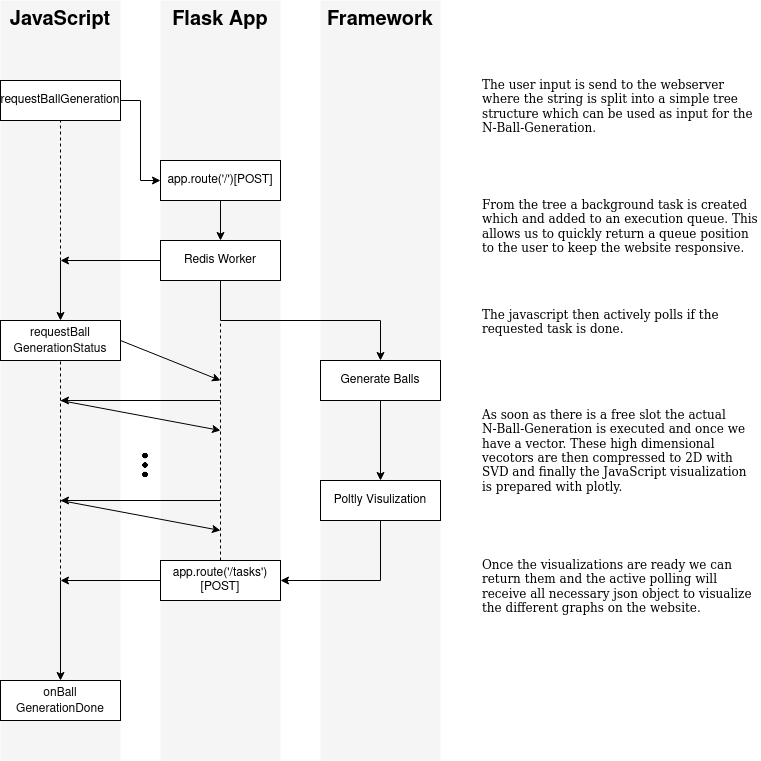
\includegraphics[width=\textwidth]{res/overview.png}
	\caption{architecture overview}
	\label{fig:overview}
\end{figure}

To get the results back to the user without the need to reload or redirect on the website we are using asynchronous AJAX requests. As soon the user either submits his input form or a file we send an AJAX request to the Web server which is immediately returned along with information of the task ID that the user has been assigned as well as which task queue this tasks resides in. With these two informations the web client can then periodically request to get a status update on his tasks progress. This update request is answered with it's current queue position or once a task is completed with the results of our plotly visualization. The realization results are passed back as a JSON file which will be parsed in the JavaScript and passed into a JavaScript plotly instance allowing us to display the different graphs.

\subsection{Flask}
\label{sec::flask}
In order to provide a easily accessible interactive demonstration, visualization and debugging tool we choose the medium of a website. As the original N-Ball embedding is implemented in Python, Flask was chosen as a web framework.  Flask is a Python based micro framework and as such does not require any additional libraries and is readily available through the python package manager. 
As is convention with a Flask application we provide HTML templates in the template folder. These templates are just the basic HTML skeleton which defines where and in which order a different graphs, input fields and text fields will be inserted on the website. The basic formatting is done through the CSS bootstrap framework. We further extend on this with our own CSS file which can be found under \textit{templates/static/css} along with the JavaScript code under \textit{templates/static/js}. 


\subsection{Redis}
\label{sec::redis}
For every input the system needs to generate the corresponding ball embeddings, save each step in the construction process, reduce the dimension of the embedding down to two dimensions for visualization and resolve overlapping that results from the dimensionality reduction. Depending on the size of the input tree this process can take anywhere from a few seconds to a few minutes. With a naïve implementation the Web server would simply do all of these tasks before sending back the response to the user. This would not only leave the user waiting with no feedback but even more importantly the server would not be reachable at all during that time frame for other users. While works well for single user it is obviously unacceptable for a publicly available website. We need to make sure that a large request will not block the Web server for everybody else for minutes, possibly even hours. Therefore we need to decouple the serving of the website from the actual computation of the ball embeddings. This is done by using a task queue.
We chose to use a commonly used task queue named Redis. This allows us to create a task queue, so when the user requests the computation of a ball embedding we add it to the task queue and immediately return to the user to tell him that we received his request and that he has been placed into the task queue. Once the task is complete the results can be sent to the users browser through AJAX without the need to refresh or redirect the website. This allows for seamless display of the results. While the website will return immediately and give the user adequate feedback this still allows a single user to effectively block the queue. As he places a large request once the Web server starts computing this task it will not work on tasks that have been requested later. In order to keep the websites response time for small requests low we introduced a second high priority queue that is reserved for small to moderate input sizes to ensure that users they want to experiment with the service will not be blocked by a single large request.
\begin{center}


\begin{tabular}{c}
\begin{lstlisting}
r = redis.Redis()
q_high = Queue("high", connection=r)
q_low  = Queue("low", connection=r)  
\end{lstlisting}
\end{tabular}
\end{center}

\subsection{Plotly} \label{plotly}
Many different graphs were introduced to the web application to fully present N-Balls embeddings and help the user understand the functionality and the concept of it. A valuable tool, on which we based our figure visualizations, was the open-source library Plotly. It helped us to present data in many different forms using the Python language. It provided us with means necessary to create scatter plots, shapes, annotations, tree plots as well as was a base for the interactive animated plot, which showed the work of N-Ball embeddings tree creation algorithm. On the end leaving the user with a possibility to observe trees with different viepoint as well as examine the construction process. Not only visualizations are showing the concept and algorithm behind but also, they are a useful tool to see if an inputted tree is correct and there are no structural problems with it. Plotly provides the graphical part of the application by allowing to present data/structures with different shapes and colors. Moreover, the library brings the graph management tools like zooming in/out. Once the plots will be generated in python with the use of Plotly they are serialized to JSON string to further be transferred to JavaScript which will manage its location and size on the website. 


\subsubsection{Paths tree}
After obtaining every keyword with its path, we combined them creating the forest of paths trees. The graph is focused on showing the user the structure and origins of the words. The clauses "is" and "is not" will indicate to which tree the word is belonging.


\begin{figure}[H]
	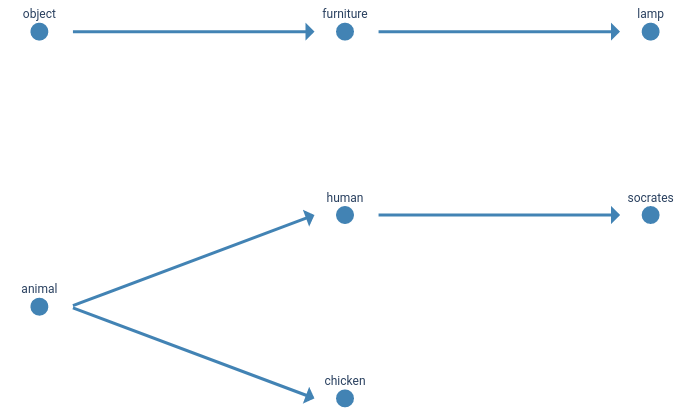
\includegraphics[width=\textwidth]{res/tree_forest.png}
	\caption{forest of words-paths trees plot}
	\label{fig:tree_forest}
\end{figure}


\subsubsection{N-Ball tree}

In the input, the algorithm receives the list of balls objects. They contain the location of the ball as well as its radius and label. With this information, the balls are transferred to the graph to show the relations between them.

\begin{figure}[H]
	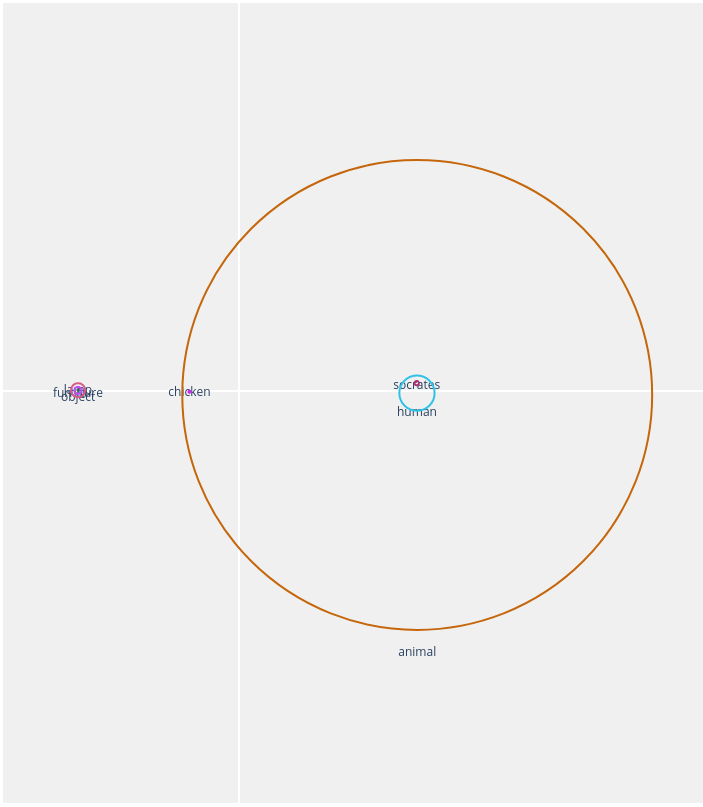
\includegraphics[width=\textwidth]{res/balls_graph.png}
	\caption{N-ball embeddings tree plot}
	\label{fig:balls_graph}
\end{figure}


\subsubsection{N-Ball tree animation}

Our animation is triggered by two buttons: "Next step", "Previous step". It is based on the same algorithm as the generation of N-Ball tree. With the difference that in this graph the animation algorithm will generate the same amount of N-Ball tree graphs as the amount of the steps of the balls generation algorithm took.  Therefore the received input for plots generation is a list of steps where every step contains a list of balls with its arguments.

We can distinguish different stages of ball creation:
\begin{itemize}
	\item initialize: prints the new ball to the plot.
	\item  contain: changes the position of the balls in relation to each other that one ball will be contained in another
	\item  separate: changes th position of the balls in relation to each other that the balls will be separated and will not contain each other
\end{itemize}

\begin{figure}[H]
	\begin{tabular}{cc}
	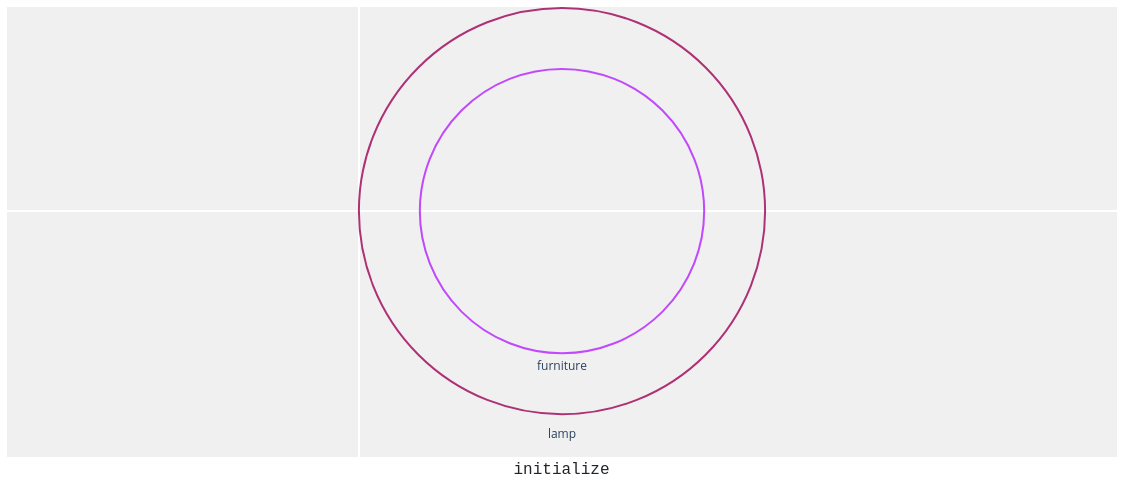
\includegraphics[width=55mm]{res/animation1.png} & 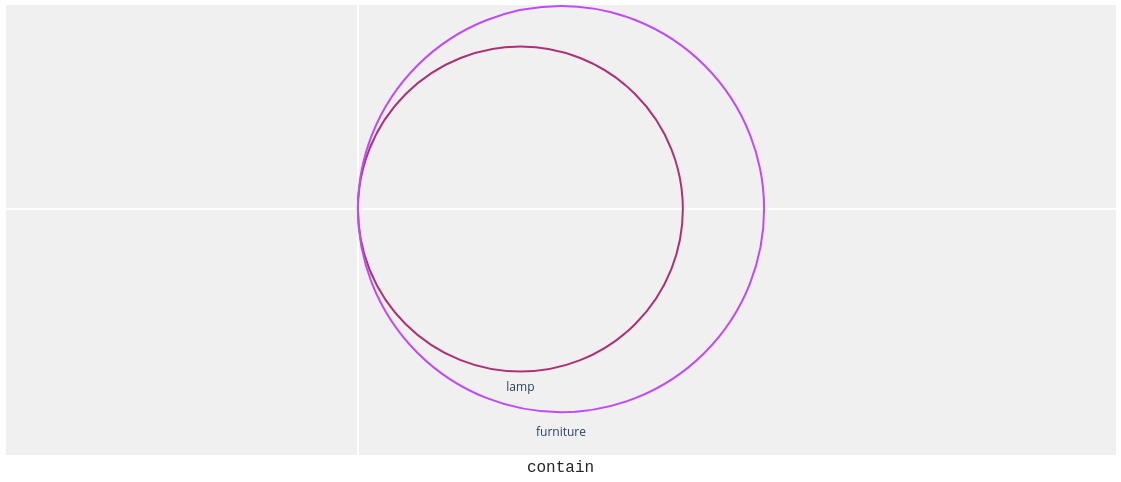
\includegraphics[width=55mm]{res/animation2.png} \\
	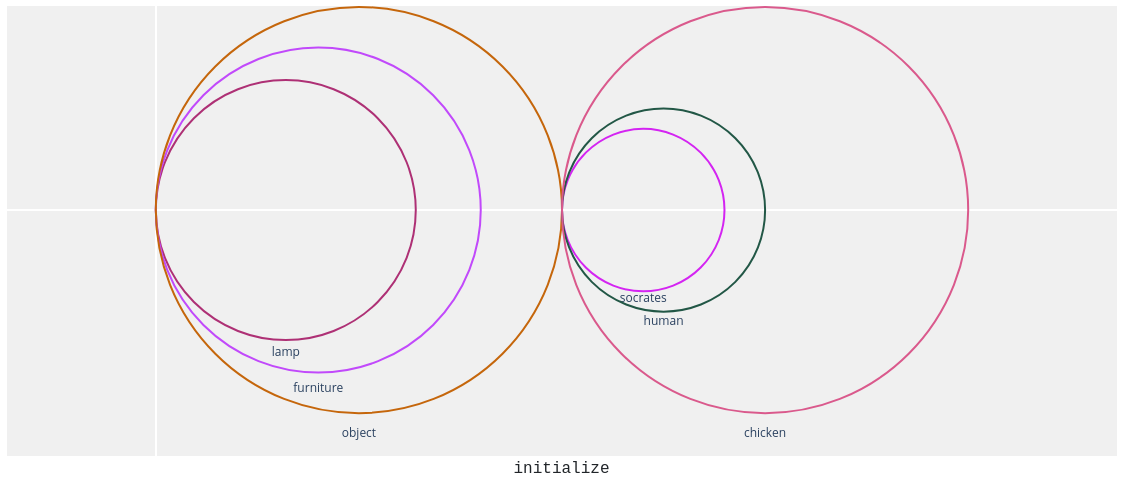
\includegraphics[width=55mm]{res/animation3.png} & 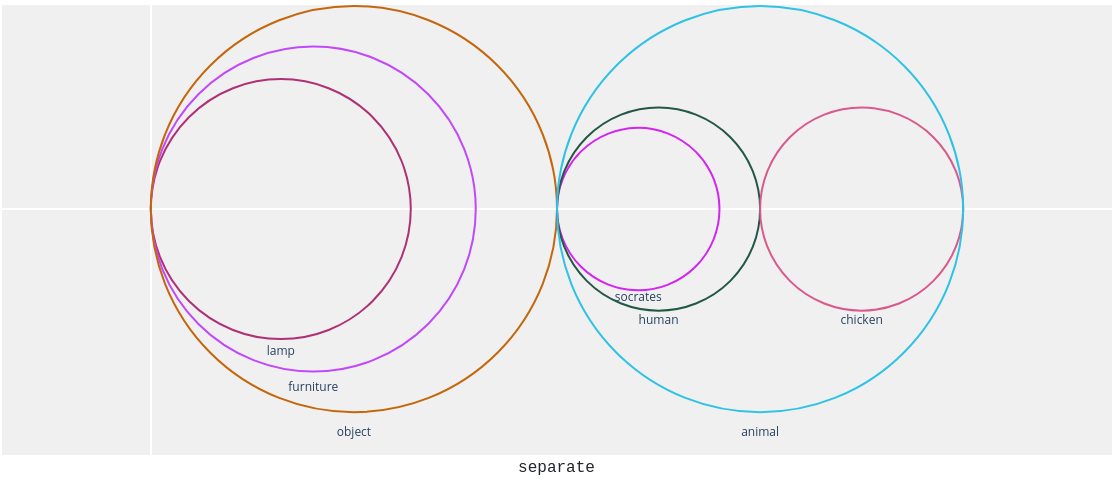
\includegraphics[width=55mm]{res/animation4.png} \\
	\end{tabular}
	\caption{N-Ball tree animation plot. Step 3,4, }
	\label{fig:animation}
\end{figure}

\subsection{Word sense exploration}
The initial scope of the project was planning to extract the tree structure that is needed to compute the N-Ball embedding from wordnet. WordNet is a database that collects semantic relationships between English words. The user would have simply given a list of input words that he wishes to explore and we would get all possible connections between these words from WordNet. 
Right away one issue arises as many words in the English language change their meaning depending on the context they are used in. For example the word tank can be used to describe a fillable container or the armored vehicle used in most modern wars. To resolve this ambiguity WordNet attaches a word sense notation to each word. In our example tank.n.01 and tank.n.02 as well as many more. Every entry will now uniquely respond to one word sentence of the word tank. This notation uses .n to denote nouns and .v to denote verbs. After this separation it simply enumerates all existing word sentences. Now that the meaning of each entry is fixed WordNet can assign meaningful relationships between these unique entities. 

However it might confuse the user that he provided a single word tank but the system presents him with multiple versions of the same word. To make this more understandable we build a word sense Explorer that shows the user which word sentences exist for every input word. Further we would give a definition of the selected word sense along with a single branch going back from this entity up to the root node that is being visualized.

\begin{figure}[H]
	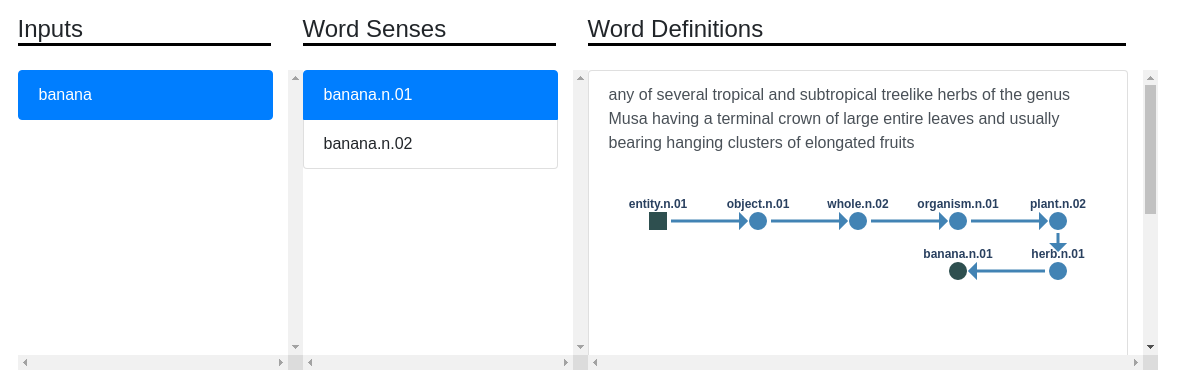
\includegraphics[width=\textwidth]{res/word-sense.png}
	\caption{words senses Explorer}
	\label{fig:word-sense}
\end{figure}



Later during the project it was decided to shift the focus of the project towards visual debugging and this feature was discontinued.

\section{User Interaction}

\subsection{Page overview}
The page was created in a simple and intuitive manner so the user can have a clear intuition of the functionalities as well as understand its purpose. The color scheme was chosen based on university colors. 

Page is divided into: 
\begin{itemize}
	\item header with logo, title and contact button,
	\item input box with two methods of submission,
	\item main body with the generated results.
\end{itemize}


\begin{figure}[H]
	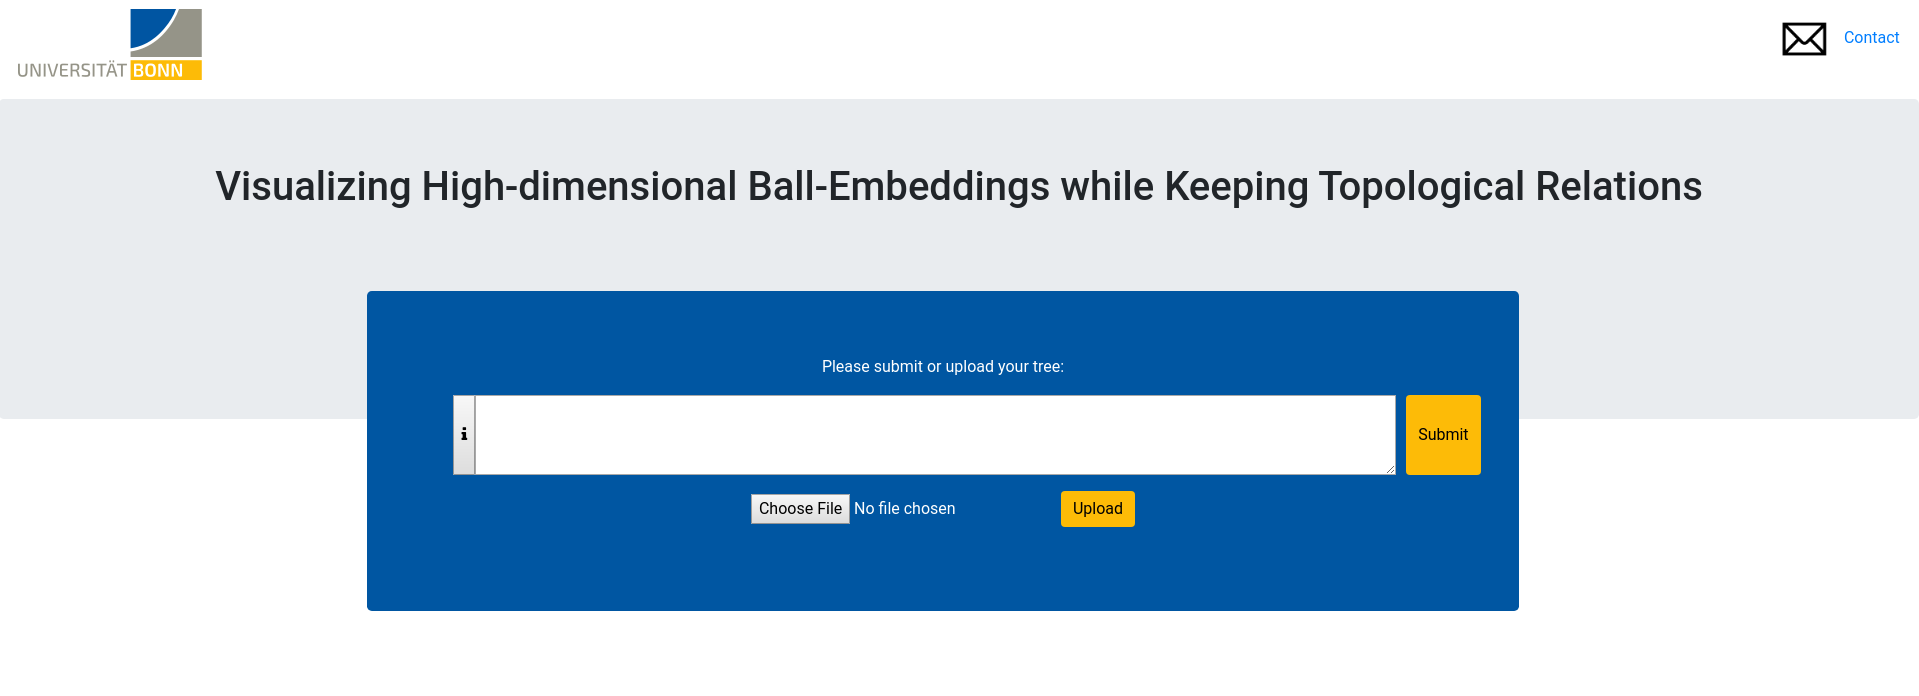
\includegraphics[width=\textwidth]{res/page.png}
	\caption{web page overview}
	\label{fig:page}
\end{figure}


\subsubsection{Contact}
We provided the contact possibility if there are any questions or remarks. Contact button transfers automatically to the mail service with pre-filled mail address.

\subsubsection{Info}
Clicking the little button with "i" icon, close to a text box, triggers the opening of the pop up which includes the explanatory information about the input and its example in a clear way that the user knows how to construct his/her own tree. 

\subsection{Input}
The application provides two ways for input. Its purpose is to ease the user interaction and give the option depending on the size of the query. 

\begin{itemize}
	\item Text box: user writes manually the input. Created with the thought of small inputs as well as dedicated to page exploration. Text box can accommodate long strings however its main purpose is small query testing. The generation of the output is followed after providing the proper input and clicking on the submit button next to the text box.
	\item  File upload: function dedicated to pre-written texts, big queries as well as additional information like users own ball embeddings. Designed with the thought to ease the process of creation of the query and faster tree structure testing. Users can use the editor of their own choice for flexibility and then upload files in the text format as well as JSON. 
\end{itemize}


\subsection{Output}
After input submission website shows three different plots. While the graphs calculating and generation take time depending on the size of the query, user is provided with waiting animation to indicate the process. 

\begin{figure}[H]
	\centering
	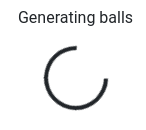
\includegraphics[scale=0.5]{res/waiting.png}
	\caption{waiting annimation}
	\label{fig:waiting}
\end{figure}


Plots provide user with different intake and presentation of the inputted tree:
\begin{itemize}
	\item Path tree: shows a forest of trees from a structural perspective. User can have an overview of what are exact word paths and how they interact with each other.
	\item N-Ball tree: shows the ball embeddings and their relation between each other.
	\item N-Ball tree animation: shows the process of ball embeddings creation. User is provided with two buttons to move to the next and previous step of the application as well as is provided with titles explaining the step.	
\end{itemize}

All the plots are zoomable with the scrooll wheel. 
For more information about the plots look to section \ref{plotly}.

\section{Extentions and Faults}
\subsection{Visulization of construction history}
Initially the idea for the project included a visual debugger. Many references to visual debugging may still persist in the code base. When using an actual debugger in any programming language the program executes up to a breakpoint from which the programmer can decide to step through the code instruction by instruction. For a visual debugger of the ball embedding process in theory you wish to achieve the same but on a more abstract level. For each entry in the tree a sphere needs to be constructed and the extended word vector needs to be adjusted. The debugger should ideally display every adjustment made to the word vector that the developer can see if his algorithm is misbehaving. This approach generates three major problems. 

First is the system actually works like a traditional debugger at the time of visualizing a D debugging step t we can only access the ball embedding's that have been computed previously. However as explained in REFERENCE before we can do the actual visualization we have to reduce the dimensionality of the ball embedding. The projection to the 2D space will obviously change with every additional data point that is added. Therefore the position and even size of the 2D projection of a ball embedding will not be consistent throughout the different debugging steps. This is quite obviously very irritating and will make a productive use of the visual debugging tool very difficult.
Second if the user has the ability to trigger the step in the construction process this has to be tightly integrated with the specific ball embedding framework. Therefore the web service would be confined to the specific ball embedding framework used in this project. 
Third the ball embedding framework that this project is based on is not designed to pause the construction process and much less to allow for adjustments before the next ball embedding is constructed. As such this would require significant rewriting of the ball embedding framework and is as such out of the scope of this project.

Instead we decided to visualize a construction history or another words simple log of the debugging steps as a list. This has the advantage that we can provide a simple JSON format of how this construction history should be saved and then our visualization can be used with any ball embedding framework as well as the one used here.
\subsection{Webserver deployment}
For the testing of the web service we have used the built in Web server that is provided by flask. If the service will be actually deployed this needs to be changed to a proper Web server as is explained in the flask tutorials.
\subsection{Result Notification}
Currently we require the user to keep the website open until his request has been completed. Some users may only be interested in the resulting ball embedding but we currently do not offer any ability to download them directly. For these users there should be the possibility of a simple download button to retrieve the ball embedding for exploration on their own system. Further these users may also use our service to compute ball embedding's of larger input trees. For these larger requests the user would be required to provide his email address and once the task is finished we can send him a download link for his ball embedding. Further this would allow us to acquire the email addresses of persons interested in our research.


\section{Developer Notes and Insights}
During the embedding generation the web server generates some files. While they may not be of concern for the end user observing the website it is helpful for future developers of the application to understand their format.

\subsection{Contents of out folder}
When running the application a new folder is created in the directory $out/$. The embedding algorithm we based our web interface in then generates the following files in it

\begin{center}

\begin{tabular}{c}
\begin{lstlisting}
dataout/animal
dataout/chicken
dataout/human
dataout/kant
dataout/socrates
\end{lstlisting}
\end{tabular}
\\dataout/\\
 folder containing text files of the embedded words with their word vector as content

\begin{tabular}{c}
\begin{lstlisting}
*root* animal
animal human chicken
chicken
human socrates kant
socrates
kant	
\end{lstlisting}
\end{tabular}
\\children.txt
\\Contains parent child relationships between words. The first word is the parent and all following words in each line are all of it's children

\begin{tabular}{c}
\begin{lstlisting}
kant 0.1 0.2 ...
animal 0.1 -0.2 ...
chicken -0.1 0.2 ...
socrates 0.1 -0.2 ...
human 0.31 -0.2 ...
\end{lstlisting}
\end{tabular}
\\nballs.txt
\\List of words with their high dimensional embedding vector

\begin{tabular}{c}
\begin{lstlisting}
kant -0.9918952599968487 -0.12705822758005025 2.1959802804003976 0.10456600738584972
animal -0.9910574347196298 0.13343598123050138 2.216535643937416 11.283144873641081
chicken 0.9999999970703485 7.654608514690322e-05 8.739571619189181 0.05
socrates -0.9946545650656365 -0.1032583952717131 2.1896836872717182 0.10456600738584972
human -0.995477011571193 0.09500273382006987 2.1966314964104017 0.8734831363495301
\end{lstlisting}
\end{tabular}
\\reduced\_nballs\_before.txt
\\Words after their dimensionality has been reduced to 2d. The first values are the x and y coordinate, the third the radius of the circle

\begin{tabular}{c}
\begin{lstlisting}
kant -0.9918952599968487 -0.12705822758005025 2.1959802804003976 0.026192692377707306
animal -0.9910574347196298 0.13343598123050138 2.216535643937416 11.283144873641081
chicken 0.9999999970703485 7.654608514690322e-05 8.739571619189181 0.05
socrates -0.9946545650656365 -0.1032583952717131 2.1896836872717182 0.026192692377707306
human -0.995477011571193 0.09500273382006987 2.1966314964104017 0.8734831363495301
\end{lstlisting}
\end{tabular}
\\reduced\_nballs\_after.txt
\\While reducing the dimensionality some child parent relationships might get violated. Here are the words after fixing.

\begin{tabular}{c}
\begin{lstlisting}
*root* 1 0 0 0 0 0 0 0 0 0 0 0 0 0 0
animal 1 0 0 0 0 0 0 0 0 0 0 0 0 0 0
chicken 1 1 0 0 0 0 0 0 0 0 0 0 0 0 0
human 1 1 0 0 0 0 0 0 0 0 0 0 0 0 0
socrates 1 1 1 0 0 0 0 0 0 0 0 0 0 0 0
kant 1 1 1 0 0 0 0 0 0 0 0 0 0 0 0
\end{lstlisting}
\end{tabular}
\\small.catcode.txt
\\ ?? dunno ??


\begin{tabular}{c}
\begin{lstlisting}
*root* *root* 
animal *root* animal 
chicken *root* animal chicken 
human *root* animal human 
socrates *root* animal human socrates 
kant *root* animal human kant 

\end{lstlisting}
\end{tabular}
\\small.wordSensePath.txt
\\The first word denotes the word in question. Then we see the parent child relationship path from the root node to the word in question.

\end{center}

\subsection{File types accepted by server}
The server accepts txt and json files. They should be formated as such

\begin{center}
\begin{tabular}{c}
\begin{lstlisting}

chicken is animal
human is animal
socrates is human
kant is human


\end{lstlisting}
\end{tabular}
\\input\_file.txt
\\The text field allows the user to rapidly test various word combinations. As the length of the input increases it might prove cumbersome to enter all words by hand. To resolve this the application supports uploading text files. These files should be structured to have one sentence in the form of “CHILD is [NOT] PARENT” per line.
\end{center}

It is furthermore possible to upload log files of an N-Ball generation process that can then be viewed in the debug animation tool. A log file is an array of JSON objects that have following key:
\begin{itemize}
\item “Key”: Name of the N-Ball that an operation is performed on
\item “Op”: Code of the operation that is happening at this step in the log
\begin{itemize}
\item 0: initialize, the N-Ball is getting initialized 
\item 1: spererate, the N-Ball is getting separated from the N-Balls provided in “op\_args”
\item 2: contain, the N-Ball is being enlarged to contain the children provided in “op\_args”
\end{itemize}
\item “Op\_args”: Arguments used in the operation
\end{itemize}
[ {"key": "socrates", "op": 0, "op\_args": [], "vec": [...]}, 
{"key": "kant", "op": 0, "op\_args": [], "vec": [...]}, ... ]	


\subsection{Setup}
The setup is described in the REAMDE.md.
Start with installing redis and all required packages by running the following commands

\begin{center}
\begin{tabular}{c}
\begin{lstlisting}
apt install redis
pip install rq rq-dashboard
pip install --upgrade -r requirements.txt
\end{lstlisting}
\end{tabular}
\end{center}

Then prepare the server for handling requests with the following commands

\begin{center}
\begin{tabular}{c}
\begin{lstlisting}
rq worker high
rq worker low
python app.py
\end{lstlisting}
\end{tabular}
\end{center}


\section{Conclusion}
In this lab, we have developed a prototype of an interactive and easily portable visualization and education tool for high dimensional ball embeddings. We presented embeddings from different perspectives in order to give users a better overview of the concept. Firstly, we enabled users to generate and explore embeddings of arbitrary input word relations by providing them with plots showcasing the trees. Secondly, we visualized the generation process. Users can now clearly see in which order balls get initialized, combined, or separated by going through the sequence of plots. Both of these functions can be used to determine if the user's own embedding trees are correct. Therefore, it can be a mean to capture potential errors. Moreover, the Web application is created with a simple and intuitive manner to improve user experience. We added also a task queue to accommodate a bigger number of users at the same time. Finally, we proposed also extensions to help with a future development. 

	
	%
	% ---- Bibliography ----
	%
	% BibTeX users should specify bibliography style 'splncs04'.
	% References will then be sorted and formatted in the correct style.
	%
	% \bibliographystyle{splncs04}
	% \bibliography{mybibliography}
	
	\bibliographystyle{plain}
	\bibliography{XBib_NN,XBib} 

\end{document}
